\documentclass{article}

\usepackage[T1]{fontenc}
\usepackage{fancyhdr}
\usepackage{graphicx}
\usepackage{subfigure}
\usepackage{booktabs}
\usepackage[inline]{enumitem}
\usepackage{amsmath}
\usepackage{amssymb}
\usepackage{amsfonts}
\usepackage{hyperref}
\hypersetup{
    colorlinks=true,
    citecolor=[RGB]{0,0.5,0.5},
    urlcolor=[RGB]{0,0.5,0.5},
    linkcolor=[RGB]{0,0.5,0.5}
}
\usepackage{geometry}
\geometry{margin={0.8in,0.8in}}

\usepackage[colorinlistoftodos,prependcaption,textsize=small]{todonotes}

\begin{document}

\begin{centering}
\Large\textbf{{\sc CMPT 423 Final Exam---Winter 2025}}\\[1ex]
\large{{Deadline: April 15 at 2pm CST on Canvas}}\\
\end{centering}
\hrule

\bigskip

\begin{tabular}{lp{5in}}
\textbf{Name:} & Enter your name here. \\
\textbf{NSID:} & Enter your NSID here. \\
\end{tabular}

\section*{Submission instructions}
To complete this take-home exam, enter your answers below each question by replacing the ``\textsc{Enter your answer here and remove this line}'' section. 
Generate a .pdf file using this Latex template and submit the .pdf file as part of the Canvas Assignment ``CMPT 423 Final Exam''.

\bigskip

\noindent \textbf{Make sure to submit early and to submit often on Canvas.
As a first step, you should enter your name and NSID into this template, generate the .pdf file and submit this final without answers on Canvas.
As you work through this exam, you can always submit your answers by resubmitting on Canvas.
}

\newpage

\section{Short answer questions}

Answer each question in at most five sentences.

\subsection{Inductive bias [grade weight: 10\%]}
What is an inductive bias in a machine learning model?
Provide an explanation using an example.

\subsubsection*{Answer}
\noindent\textsc{Insert your answer here and remove this line.}

\subsection{Logistic regression [grade weight: 10\%]}
What is the purpose of the sigmoid function in logistic regression, and how does it help in modelling binary data?

\subsubsection*{Answer}
\noindent\textsc{Insert your answer here and remove this line.}

\subsection{Generalization [grade weight: 10\%]}
What is the purpose of cross-validation in machine learning, and how does it help prevent overfitting?

\subsubsection*{Answer}
\noindent\textsc{Insert your answer here and remove this line.}

\subsection{Reinforcement learning [grade weight: 10\%]}

Suppose you train a RL system, for example DQN, to play an Atari video game.
Instead of converging to a high-performing policy, DQN is stuck looping back and forth between a small number of states resulting in few rewards and poor performance.
Describe one technique to address this issue to ensure that DQN converges to an optimal policy that maximizes reward in the game.

\subsubsection*{Answer}
\noindent\textsc{Insert your answer here and remove this line.}

\newpage
\section{Maximum likelihood method [grade weight: 20\%]}

Suppose you are given a dataset of scalar values
\begin{equation*}
    \mathcal{D} = \{ x_1,...,x_n | x_i \in \mathbb{R} \}.
\end{equation*}
Assume that each $x_i \in \mathcal{D}$ is sampled i.i.d. from a normal distribution with mean $\mu$ and standard deviation one.
Derive the maximum likelihood estimate $\widehat{\mu}$ for the parameter $\mu$ given the dataset $\mathcal{D}$.

\subsubsection*{Answer}
\noindent\textsc{Insert your answer here and remove this line.}

\newpage
\section{Language models [grade weight: 20\%]}

Suppose you use the maximum likelihood method train a language model to perform list sorting.
This can be accomplished by training the model with the following prompt-response pairs
\begin{verbatim}
    Prompt:   "[ 5, 3, 6, 0 ]"
    Response: "[ 0, 3, 5, 6 ]"
\end{verbatim}
How would you create a token dataset to train a model that can sort lists and respond as in the example above?
Considering the different sequence models discussed in class, which architecture would you use and why?

\subsubsection*{Answer}
\noindent\textsc{Insert your answer here and remove this line.}


\newpage
\section{Markov Decision Processes}

Consider the following MDP with five states and an action space $\mathcal{A} = \{ a,b \}$:

\begin{center}
    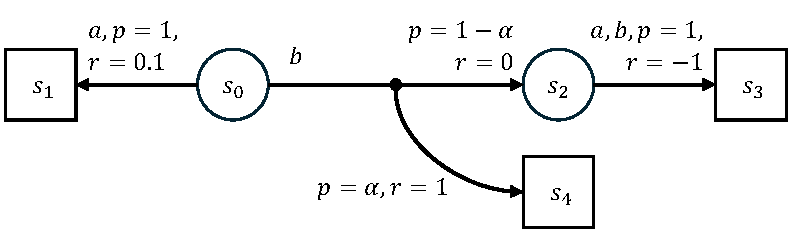
\includegraphics[scale=1]{mdp.pdf}
\end{center}

When selecting the action $a$ in state $s_0$ a reward of 0.1 is given to the agent.
When selecting the action $b$ in state $s_1$, the agent transitions to state $s_4$ with probability $\alpha$ and a reward of 1 is given.
With probability $1-\alpha$, the agent transitions to state $s_2$ and no reward is given.
From state $s_2$ the agent can select actions $a$ or $b$ again, but both actions cause a deterministic transition to state $s_3$ for which a reward of -1 is received.
The states $s_1$, $s_4$, and $s_3$ are all absorbing, meaning selecting any action at these states leads to a reward of zero and a transition back into the same state.

Depending on the setting of $\alpha$, the action $a$ or $b$ leads to a higher $\gamma$-discounted return.
In this questions you will use Q-value functions, to derive a bound for $\alpha$ where action $b$ is optimal in state $s_0$ and leads to the highest $\gamma$-discounted return.

\subsubsection*{Part A [grade weight: 6\%]}
What is the Q-value $Q(s_0,a)$ of selecting action $a$ in state $s_0$ for a discount factor $\gamma$?

\subsubsection*{Answer}
\noindent\textsc{Insert your answer here and remove this line.}

\subsubsection*{Part B [grade weight: 6\%]}
What is the Q-value $Q(s_0,b)$ of selecting action $b$ in state $s_0$ for a discount factor $\gamma$?

\subsubsection*{Answer}
\noindent\textsc{Insert your answer here and remove this line.}

\subsubsection*{Part C [grade weight: 8\%]}
For which setting of $\alpha$ is selecting action $b$ optimal?

\subsubsection*{Answer}
\noindent\textsc{Insert your answer here and remove this line.}


\end{document}